\documentclass[xcolor={dvipsnames}]{beamer}
%\documentclass[handout]{beamer} %to produce the handout

\usepackage{beamerthemeshadow}
\usepackage{graphicx}
\usepackage{textcomp}
\usepackage{xyling}
\usepackage{stmaryrd}
\usepackage{multirow}
\usepackage{pdfpages}
\usepackage[center]{caption}
\usepackage{forest}
\usepackage{caption}
\usepackage{subcaption}
\usepackage{framed}
\usepackage{pgfplots}
\usepackage[vlined]{algorithm2e}

\usetikzlibrary{decorations.pathreplacing}
\usetikzlibrary{shapes.geometric, arrows,positioning}
\tikzstyle{startstop} = [rectangle, rounded corners, minimum width=1cm, minimum height=.33cm,text centered, draw=black, fill=red!30]
\tikzstyle{process} = [rectangle, minimum width=1cm, minimum height=.33cm, text centered, draw=black, fill=orange!30]
\tikzstyle{decision} = [diamond, text centered, aspect=2, draw=black, fill=green!30]
\tikzstyle{arrow} = [thick,->,>=stealth]


\definecolor{C0}{RGB}{31,119,180}
\definecolor{C1}{RGB}{255,127,14}
\definecolor{C2}{RGB}{44,192,44}
\definecolor{C3}{RGB}{214,39,40}
\definecolor{C4}{RGB}{148,103,189}

\beamertemplatenavigationsymbolsempty 

\graphicspath{
    {images/}
}



\title{An Adaptive Index for Hierarchical\\ Database Systems}
\titlegraphic{
\includegraphics[height=.8cm]{IFIlogo.eps}}
\author{Rafael Kallis}
\institute{BSc Thesis}

\begin{document}
    \bibliographystyle{acm}
\frame{\titlepage}

%%%%%%%%%%%%%%%%%%%%%%%%%%%%%%%%%%%%%%%%%%%%%%%%%%%%%%%%%%%%%%%%%%%%%%%%%%%%%%%%%%%%%%%%%%%%%%%%%%%%%%%
%%%%%%%%%%%%%%%%%%%%%%%%%%%%%%%%%%%%%%%%%%%%%%%%%%%%%%%%%%%%%%%%%%%%%%%%%%%%%%%%%%%%%%%%%%%%%%%%%%%%%%%
%%%%%%%%%%%%%%%%%%%%%%%%%%%%%%%%%%%%%%%%%%%%%%%%%%%%%%%%%%%%%%%%%%%%%%%%%%%%%%%%%%%%%%%%%%%%%%%%%%%%%%%

\section{Introduction}
\subsection{Abstract \& Outline}
\frame{
  \begin{itemize}
    \item Skewed and update-heavy workloads trigger repeated structural index updates over a small subset of nodes to the index
    \item Informally, a frequently added or removed node is called volatile
    \item Volatile nodes decrease index update performance
  \end{itemize}
}
\frame{
    \begin{Large}
        The Workload-Aware Property Index (WAPI):
    \end{Large}
    
    \begin{itemize}
        \item Detects such volatile nodes
        \item Stops pruning volatile nodes
        \item Significantly improves update throughput
    \end{itemize}
}
\frame{
    \begin{Large}
        Unproductive nodes are an unwanted byproduct:
    \end{Large}

    \begin{itemize}
        \item When the workload changes, volatile nodes cease to be volatile
        \item They do not contribute to a query match and contain no data
        \item They waste space and slow down queries over time
    \end{itemize}

    \begin{figure}
        \centering
        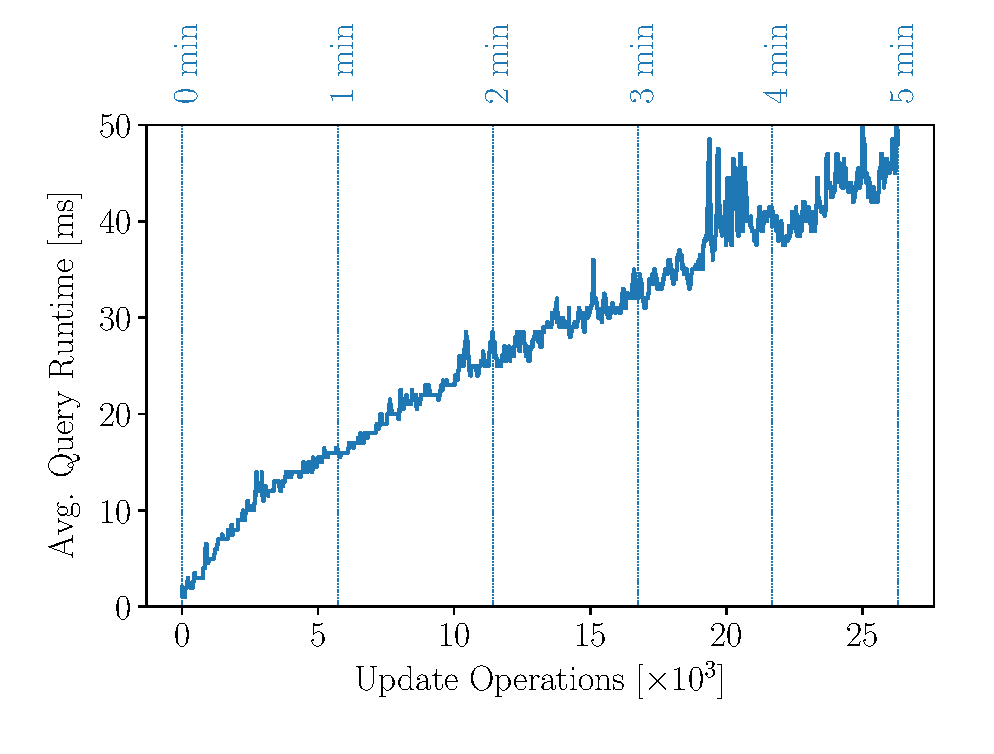
\includegraphics[height=3.8cm]{query_runtime.eps}
    \end{figure}
}
\frame{
    \begin{Large}
        In this thesis we:
    \end{Large}

    \begin{itemize}
        \item Design and implement two solutions in order to mitigate unproductive nodes
        \item Analyze factors impacting the production of unproductive nodes
        \item Empirically evaluate and compare our two solutions
    \end{itemize}
}
\subsection{Example}
\frame{
    \centering
    \Large
    Example: e-commerce platform
}
\frame{
    \centering
    Hierarchical database for an e-commerce platform

    \footnotesize
    \begin{figure}
        \begin{forest}
            [
            [index]
            [,phantom]
            [,phantom]
            [products
            [consumer
            [$\alpha$]
            [$\beta$]
            ]
            [enterprise
            [$\gamma$]
            ]
            ]
            ]
        \end{forest}
    \end{figure}
}
\frame{
    \centering
    HTML pre-rendering 

    \footnotesize
    \begin{figure}
      \begin{subfigure}{.4\textwidth}
        \begin{forest}
          [
          [index]
          [,phantom]
          [,phantom]
          [products
          [consumer
          [$\alpha$]
          [$\beta$]
          ]
          [enterprise
          [$\gamma$]
          ]
          ]
          ]
        \end{forest}
        \vspace{2cm}
      \end{subfigure}
      \begin{subfigure}{.1\textwidth}
        \centering
        $\longrightarrow$
      \end{subfigure}
      \begin{subfigure}{.4\textwidth}
        \begin{forest}
            [
            [index
            [render
            [now
            [products
            [consumer
            [$\alpha$ \\ render:now, align=center, base=bottom]
            ]
            ]
            ]
            ]
            ]
            [products
            [consumer
            [$\alpha$ \\ render:now, align=center, base=bottom]
            [$\beta$]
            ]
            [enterprise
            [$\gamma$]
            ]
            ]
            ]
        \end{forest}
      \end{subfigure}
    \end{figure}
}
%\frame{
    %\begin{large}
        %A Content Management System's (CMS) workload is:
    %\end{large}
    
    %\begin{itemize}
        %\item skewed
        %\item update-heavy
        %\item changing
    %\end{itemize}

    %%CMSs frequently use a job-queuing system that has the noted characteristics.
%}
%\frame{
    %Skewed workload: small subset of nodes gets frequently updated
    %\vspace{1cm}
    %\begin{figure}
        %\centering
        %\begin{subfigure}{0.30\textwidth}
            %\centering
            %\scriptsize
            %\begin{forest}
                %[,circle,draw,fill=YellowOrange
                %[,circle,draw,fill=YellowOrange
                %[,circle,draw,fill=YellowOrange
                %]
                %[,circle,draw,fill=YellowOrange
                %[,circle,draw,fill=YellowOrange]
                %[,phantom]
                %]
                %]
                %[,circle,draw,fill=YellowOrange
                %[,phantom]
                %[,circle,draw,fill=YellowOrange
                %[,circle,draw,fill=YellowOrange]
                %[,circle,draw,fill=YellowOrange]
                %]
                %]
                %]
            %\end{forest}

            %No skew
        %\end{subfigure}
        %\begin{subfigure}{0.30\textwidth}
            %\centering
            %\scriptsize
            %\begin{forest}
                %[,circle,draw,fill=Yellow
                %[,circle,draw,fill=Yellow
                %[,circle,draw,fill=Yellow
                %]
                %[,circle,draw,fill=Yellow
                %[,circle,draw,fill=Orange]
                %[,phantom]
                %]
                %]
                %[,circle,draw,fill=Orange
                %[,phantom]
                %[,circle,draw,fill=Yellow
                %[,circle,draw,fill=Red]
                %[,circle,draw,fill=Orange]
                %]
                %]
                %]
            %\end{forest}

            %Normal skew
        %\end{subfigure}
        %\begin{subfigure}{0.30\textwidth}
            %\centering
            %\scriptsize
            %\begin{forest}
                %[,circle,draw,fill=Yellow
                %[,circle,draw,fill=Yellow
                %[,circle,draw,fill=Yellow
                %]
                %[,circle,draw,fill=Yellow
                %[,circle,draw,fill=Yellow]
                %[,phantom]
                %]
                %]
                %[,circle,draw,fill=Yellow
                %[,phantom]
                %[,circle,draw,fill=Yellow
                %[,circle,draw,fill=Red]
                %[,circle,draw,fill=Red]
                %]
                %]
                %]
            %\end{forest}

            %High skew
        %\end{subfigure}
    %\end{figure}
%}
%\frame{
    %Changing workload: as time passes, hotspots change
    %\vspace{1cm}
    %\begin{figure}
        %\centering
        %\begin{subfigure}{0.20\textwidth}
            %\centering
            %\scriptsize
            %\begin{forest}
                %[,circle,draw,fill=Yellow
                %[,circle,draw,fill=Yellow
                %[,circle,draw,fill=Orange
                %]
                %[,circle,draw,fill=Yellow
                %[,circle,draw,fill=Red]
                %[,phantom]
                %]
                %]
                %[,circle,draw,fill=Yellow
                %[,phantom]
                %[,circle,draw,fill=Yellow
                %[,circle,draw,fill=Yellow
                %[,circle,draw,fill=Yellow]
                %[,circle,draw,fill=Yellow]
                %]
                %[,circle,draw,fill=Orange]
                %]
                %]
                %]
            %\end{forest}
        %\end{subfigure}
        %\begin{subfigure}{0.10\textwidth}
            %\centering
            %$\longrightarrow$
        %\end{subfigure}
        %\begin{subfigure}{0.20\textwidth}
            %\centering
            %\scriptsize
            %\begin{forest}
                %[,circle,draw,fill=Yellow
                %[,circle,draw,fill=Yellow
                %[,circle,draw,fill=Yellow
                %]
                %[,circle,draw,fill=Yellow
                %[,circle,draw,fill=Yellow]
                %[,phantom]
                %]
                %]
                %[,circle,draw,fill=Orange
                %[,phantom]
                %[,circle,draw,fill=Yellow
                %[,circle,draw,fill=Yellow
                %[,circle,draw,fill=Orange]
                %[,circle,draw,fill=Red]
                %]
                %[,circle,draw,fill=Orange]
                %]
                %]
                %]
            %\end{forest}
        %\end{subfigure}
        %\begin{subfigure}{0.10\textwidth}
            %\centering
            %$\longrightarrow$
        %\end{subfigure}
        %\begin{subfigure}{0.20\textwidth}
            %\centering
            %\scriptsize
            %\begin{forest}
                %[,circle,draw,fill=Yellow
                %[,circle,draw,fill=Yellow
                %[,circle,draw,fill=Orange
                %]
                %[,circle,draw,fill=Yellow
                %[,circle,draw,fill=Yellow]
                %[,phantom]
                %]
                %]
                %[,circle,draw,fill=Yellow
                %[,phantom]
                %[,circle,draw,fill=Yellow
                %[,circle,draw,fill=Red
                %[,circle,draw,fill=Orange]
                %[,circle,draw,fill=Yellow]
                %]
                %[,circle,draw,fill=Yellow]
                %]
                %]
                %]
            %\end{forest}
        %\end{subfigure}
    %\end{figure}
%}
%\frame{
    %\large
    %CMSs usually use a job-queuing system that has the noted characteristics
%}
\subsection{Workload-Aware Property Index}
\frame{
    \centering
    \Large
   Workload-Aware Property Index 
}
\frame{
    \frametitle{Hierarchical Database with WAPI}
    \begin{figure}
        \centering
        \scriptsize
        \begin{forest}
            [
            [index
            [render
            [now
            [products
            [consumer
            [$\alpha$ \\ render:now, align=center, base=bottom, name=i_node] {
                \draw[<-,gray] (.north west)--++(-2em,1em)
                node[anchor=east]{\textit{Matching Node}};
            }
            ]
            [,phantom]
            ]
            ]
            ]
            ] {
                \draw[<-,gray] (.south west)--++(-3em, -1em)
                node[anchor=east]{\textit{Index Subtree Root}};
            }
            [products
            [consumer
            [$\alpha$ \\ render:now, align=center, base=bottom, name=c_node]
            [$\beta$]
            ]
            [enterprise
            [$\gamma$]
            ]
            ] {
                \draw[<-,gray] (.south east)--++(3.5em, -1em)
                node[anchor=west]{\textit{Content Subtree Root}};
            }
            ]
            \draw[->,dotted] (i_node) to[out=east, in=south] node[gray,midway,right]{\textit{corresponding content node}} (c_node);
        \end{forest}
    \end{figure}
}
\frame{
    We denote node $n$'s property $k$ as $n[k]$ and node $n$'s descendants as
    $desc(n)$.

    \begin{definition}[CAS Query]
        Given node $m$, property $k$ and value $v$, a CAS query
        $Q(k,v,m)$ returns all descendants of $m$ which have $k$ set to $v$, i.e.,
        $$ Q(k,v,m) = \{ n | n \in desc(m) \land n[k] = v\} $$
    \end{definition}
}
%\frame{
    %Volatility is the measure which is used by the WAPI in order to distinguish
    %whether to remove a node or not from the index.
    %Wellenzohn et al.~\cite{KW17} propose to look at the recent transactional
    %workload to check whether a node $n$ is volatile.
%}
%\frame{
    %\begin{definition}[Volatility Count]
        %The volatility count $vol(n)$ of index node $n$ on database instance $O_i$, is the number of
        %times node $n$ was added or removed from snapshots contained in a Sliding
        %Window of Length $L$ over history $H_i$, i.e.,
        %\vspace{3mm}
        %\begin{align*}
            %vol(n) = | \{ G^b | G^b \in H_i \land t(G^b) \in [t_n-L+1, t_n] \land \exists G^a[ \\
                %\qquad G^a = pre(G^b) \land ([n^a \notin N(G^a) \land n^b \in N(G^b)]\lor \\
            %\qquad [n^a \in N(G^a) \land n^b \notin N(G^b)] )]\} |
        %\end{align*}
    %\end{definition}
%}
\frame{
    \begin{definition}[Volatile Node]
        Index node $n$ is volatile iff $n$'s volatility count is greater or equal than 
        the volatility threshold $\tau$, i.e.,
        \vspace{3mm}
        $$ volatile(n) \iff vol(n) \geq \tau $$
    \end{definition}

    \centering
    \footnotesize
    \begin{itemize}
        \item volatility count $vol(n)$ is the number of insertions and deletions of node $n$ inside
            a sliding window.
    \end{itemize}
}
\frame{
    \frametitle{Index nodes becoming volatile}
    \begin{figure}
        \begin{subfigure}{0.2\textwidth}
            \centering 
            \tiny
            \begin{forest}
                [
                [$i$
                [,phantom]
                ]
                [,phantom]
                [,phantom]
                [$p$
                [$c$
                [$\alpha$]
                [$\beta$]
                ] 
                [,phantom]
                [$e$
                [$\gamma$]
                ]
                ]
                ]
            \end{forest}

            \vspace{21mm}
        \end{subfigure}
        \begin{subfigure}{.05\textwidth}
            \centering
            $\longrightarrow$
        \end{subfigure}
        \begin{subfigure}{.3\textwidth}
            \centering
            \tiny
            \begin{forest}
                [
                [$i$
                [rend, color=RoyalBlue
                [now, color=RoyalBlue
                [$p$, color=RoyalBlue
                [$c$, color=RoyalBlue
                [$\alpha$ \\ rend:now, color=RoyalBlue, align=center, base=bottom]
                ]
                ]
                ]
                ]
                ]
                [$p$
                [$c$
                [$\alpha$ \\ rend:now, align=center, base=bottom]
                [$\beta$]
                ]
                [$e$
                [$\gamma$]
                ]
                ]
                ]
            \end{forest}
        \end{subfigure}
        \begin{subfigure}{.05\textwidth}
            \centering
            $\longrightarrow$
        \end{subfigure}
        \begin{subfigure}{0.3\textwidth}
            \centering 
            \tiny
            \begin{forest}
                [
                [$i$
                [rend, color=RoyalBlue
                [now, color=RoyalBlue
                [$p$, color=RoyalBlue
                [$c$, color=RoyalBlue
                [$\alpha$, color=RoyalBlue]
                ]
                ]
                ]
                ]
                ]
                [$p$
                [$c$
                [$\alpha$]
                [$\beta$]
                ]
                [$e$
                [$\gamma$]
                ]
                ]
                ]
            \end{forest}

            \vspace{3mm}
        \end{subfigure}
    \end{figure}

    \tiny
    \textcolor{RoyalBlue}{volatile}
}
\section{Unproductive Nodes}
\subsection{Introduction}
\frame{
    \centering
    \Large
    Unproductive Nodes
}
%\frame{
    %\begin{itemize}
        %\item When nodes are volatile, their volatility count has to be at least $\tau$
        %\item Time passes and the database workload changes
        %\item Insertions and deletions that increased the volatility count drop out of the sliding window
        %\item If the volatility count drops below threshold $\tau$, the node ceases to be volatile
        %\item If the same holds for the node's descendants, we call the node and its descendants unproductive
    %\end{itemize}
%}
\frame{
    \frametitle{Index nodes becoming unproductive}
    \begin{figure}
        \begin{subfigure}{0.35\textwidth}
            \centering 
            \tiny
            \begin{forest}
                [
                [i
                [rend, color=RoyalBlue
                [now, color=RoyalBlue
                [p, color=RoyalBlue
                [c, color=RoyalBlue
                [$\alpha$, color=RoyalBlue]
                ]
                %[,phantom]
                %[,phantom]
                ]
                ]
                ]
                ]
                [p
                [c
                [$\alpha$]
                [$\beta$]
                ]
                [,phantom]
                [e
                [$\gamma$]
                ]
                ]
                ]
            \end{forest}
        \end{subfigure}
        \begin{subfigure}{.1\textwidth}
            \centering
            $\longrightarrow$
        \end{subfigure}
        \begin{subfigure}{.35\textwidth}
            \centering
            \tiny
            \begin{forest}
                [
                [i
                [rend, color=Orange
                [now, color=Orange
                [p, color=Orange
                [c, color=Orange
                [$\alpha$, color=Orange]
                ]
                %[e, color=RoyalBlue
                %[$\gamma$ \\ rend:now, color=RoyalBlue, align=center, base=bottom]
                %]
                ]
                ]
                ]
                ]
                [,phantom]
                [p
                [c
                [$\alpha$]
                [$\beta$]
                ]
                [e
                [$\gamma$]
                ]
                ]
                ]
            \end{forest}
        \end{subfigure}
    \end{figure}

    \begin{center}
      \footnotesize
      Volatile nodes might cease to be volatile and become unproductive
    \end{center}

    \tiny
    \textcolor{RoyalBlue}{volatile}

    \textcolor{Orange}{unproductive}
}
\frame{
    \begin{definition}[Unproductive Node]
        Index node $n$ is unproductive iff $n$, and any descendant of
        $n$, is neither matching, nor volatile, i.e.,
        \begin{align*}
            unproductive(n) \iff \forall m (m \in (\{n\} \cup desc(n)) \implies \\
            (\neg matching(m) \land \neg volatile(m)))
        \end{align*}
    \end{definition}
}
\frame{
    \centering
    \scriptsize
    \begin{forest}
        [
        [i
        [rend
        [now
        [p
        [c, color=Orange
        [$\alpha$, color=Orange]
        ]
        [e
        [$\gamma$ \\ rend:now, align=center, base=bottom]
        ]
        ]
        ]
        ]
        ]
        [,phantom]
        [p
        [c
        [$\alpha$]
        [$\beta$]
        ]
        [e
        [$\gamma$ \\ rend:now, align=center, base=bottom]
        ]
        ]
        ]
    \end{forest}

    $$ unproductive(n) \iff \forall m (m \in (\{n\} \cup desc(n)) \implies (\neg matching(m) \land \neg volatile(m))) $$

    \raggedright
    \tiny
    \textcolor{RoyalBlue}{volatile}

    \textcolor{Orange}{unproductive}
}
\frame{
    The number of unproductive nodes depends on: 
    \begin{itemize}
        \item Volatility threshold $\tau$
        \item Sliding window length $L$
        \item Workload skew $s$
        \item Update operations per second
    \end{itemize}
}
\frame{
    Unproductive index node cleaning, we propose:
    \begin{itemize}
        \item Periodic Garbage Collection (GC)
        \item Query-Time Pruning (QTP)
    \end{itemize}
}
\subsection{Periodic Garbage Collection}
\frame{
    \centering
    \large
    Periodic Garbage Collection (GC)
}
\frame{
    \frametitle{Periodic GC}
    Main idea:

    \begin{itemize}
        \item Background process
        \item Periodically traverse the whole index subtree
        \item Prune any visited unproductive node
    \end{itemize}
}
%\frame{
    %\frametitle{Periodic GC}
    %\begin{algorithm}[H]
        %\TitleOfAlgo{GarbageCollect}
        %\DontPrintSemicolon
        %\For{node $n \in desc(\texttt{/i})$ in postorder tree walk}{
            %\If{$chd(n) = \emptyset \land \neg matching(n) \land \neg volatile(n)$}{
                %delete node $n$\;
            %}
        %}
    %\end{algorithm}
%}
\frame{
    \frametitle{Periodic GC}
    \begin{figure}
        \begin{subfigure}{0.35\textwidth}
            \centering
            \tiny
            \begin{forest}
                [
                [i
                [rend
                [now
                [p
                [c, color=Orange
                [$\alpha$, color=Orange]
                ]
                [e
                [$\gamma$ \\ rend:now, align=center, base=bottom]
                ]
                ]
                ]
                ]
                ]
                [,phantom]
                [p
                [c
                [$\alpha$]
                [$\beta$]
                ]
                [e
                [$\gamma$ \\ rend:now, align=center, base=bottom]
                ]
                ]
                ]
            \end{forest}
        \end{subfigure}
        \begin{subfigure}{0.1\textwidth}
            \centering
            $\longrightarrow$
        \end{subfigure}
        \begin{subfigure}{0.35\textwidth}
            \centering
            \tiny
            \begin{forest}
                [
                [i
                [rend
                [now
                [p
                [,phantom]
                [,phantom]
                [e
                [$\gamma$ \\ rend:now, align=center, base=bottom]
                ]
                ]
                ]
                ]
                ]
                [,phantom]
                [p
                [c
                [$\alpha$]
                [$\beta$]
                ]
                [e
                [$\gamma$ \\ rend:now, align=center, base=bottom]
                ]
                ]
                ]
            \end{forest}
        \end{subfigure}
    \end{figure}    
    
    \raggedright
    \tiny
    \textcolor{RoyalBlue}{volatile}
}
\subsection{Query-Time Pruning}
\frame{
    \centering
    \large
    Query-Time Pruning (QTP)
}
\frame{
    \frametitle{Query-Time Pruning}
    Main idea:

    \begin{itemize}
        \item Prune unproductive nodes during query execution
        \item Piggybacking on query execution
        \item Adds overhead on query runtime
        \item Avoids unnecessary full index traversals
        \item We traverse a part of the index subtree and prune any visited unproductive node
    \end{itemize}
}
%\frame{
    %\frametitle{Query-Time Pruning}
    %\begin{algorithm}[H]
        %\TitleOfAlgo{QueryQTP}
        %\DontPrintSemicolon
        %\KwData{Query $Q(k, v, m)$, where $k$ is a property, $v$ a value and $m$ (=
            %$\texttt{/}\lambda_1\texttt{/}\dots\texttt{/}\lambda_d$) a
        %content node's path.}
        %\KwResult{A set of nodes satisfying $Q(k,v,m)$}
        %$r \longleftarrow \emptyset$\;
        %\For{node $n \in
            %desc(\texttt{/i/k/v/}\lambda_1\texttt{/}\dots\texttt{/}\lambda_d)$ in postorder tree walk}{
            %\uIf{$matching(n)$}{
                %$r \longleftarrow r \cup \{ *n \}$\;
            %}
            %\ElseIf{$chd(n) = \emptyset \land \neg volatile(n)$}{
                %delete node $n$
            %}
        %}
        %\Return{r}\;
    %\end{algorithm}
%}
\frame{
    \frametitle{Query-Time Pruning}
    \vspace{-1cm}
    \begin{figure}
        \centering
        \begin{subfigure}{0.40\textwidth}
            \centering 
            \tiny
            \begin{forest}
                [
                [i
                [rend
                [now
                [p
                [c, tikz={\node [draw,red,inner sep=0,fit to=tree]{};}
                [$\alpha$ \\ rend:now, align=center, base=bottom]
                [$\beta$ \\ \vspace{-1mm}, color=Orange, align=center, base=bottom]
                ]
                [e, color=Orange
                [$\gamma$, color=Orange]
                ]
                ]
                ]
                ]
                ]
                [p
                [c
                [$\alpha$ \\ rend:now, align=center, base=bottom]
                [$\beta$ \\ \vspace{-1mm}, align=center, base=bottom]
                ]
                [e
                [$\gamma$]
                ]
                ]
                ]
            \end{forest}
        \end{subfigure}
        \begin{subfigure}{0.1\textwidth}
            \centering
            $\longrightarrow$
        \end{subfigure}
        \begin{subfigure}{0.40\textwidth}
            \centering 
            \tiny
            \begin{forest}
                [
                [i
                [rend
                [now
                [p
                [c
                [$\alpha$ \\ rend:now, align=center, base=bottom]
                [,phantom]
                [,phantom]
                ]
                [e, color=Orange
                [$\gamma$, color=Orange]
                ]
                ]
                ]
                ]
                ]
                [p
                [c
                [$\alpha$ \\ rend:now, align=center, base=bottom]
                [$\beta$ \\ \vspace{-1mm}, align=center, base=bottom]
                ]
                [e
                [$\gamma$]
                ]
                ]
                ]
            \end{forest}
        \end{subfigure}
    \end{figure}
    \centering
    \footnotesize
    $Q(\texttt{render},\texttt{now},\texttt{/products/consumer})$

    \raggedright
    \tiny
    \textcolor{Orange}{unproductive}
}
\section{Experimental Evaluation}
\frame{
    \centering
    \large
    Experimental Evaluation
}
\frame{
    \centering
    Experiments are run on the hierarchical database system \\
    Apache Jackrabbit Oak

    \begin{figure}
        
\includegraphics[height=2cm]{oak_logo.png}
    \end{figure}
}
\frame{
    \frametitle{Datasets}
    \begin{itemize}
        \item Datasets resemble the content subtree
    \end{itemize}
    \begin{figure}
        \centering
        \hspace{-1cm}
        \begin{subfigure}{0.59\linewidth}
            \centering
            \caption{Synthetic}
            \tiny
            \begin{forest}
                [,circle,draw
                [,circle,draw
                [,circle,draw
                [,circle,draw
                [,circle,draw]
                [,circle,draw] 
                ]
                [,circle,draw
                [,circle,draw]
                [,circle,draw]
                ]
                ]    
                [,circle,draw
                [,circle,draw
                [,circle,draw]
                [,circle,draw] 
                ]
                [,circle,draw
                [,circle,draw]
                [,circle,draw]
                ]
                ] 
                ]
                [,circle,draw
                [,circle,draw
                [,circle,draw
                [,circle,draw]
                [,circle,draw] 
                ]
                [,circle,draw
                [,circle,draw]
                [,circle,draw]
                ]
                ]
                [,circle,draw
                [,circle,draw
                [,circle,draw]
                [,circle,draw] 
                ]
                [,circle,draw
                [,circle,draw]
                [,circle,draw]
                ]
                ]  
                ]
                ]
            \end{forest}

            \centering
            \footnotesize
            $2^{20} \approx 10^6$ nodes
        \end{subfigure}
        \begin{subfigure}{0.39\linewidth}
            \centering
            \caption{Dell}
            \tiny
            \begin{forest}
                [,circle,draw
                [,phantom]
                [,circle,draw
                [,circle,draw
                [,circle,draw]
                [,circle,draw
                [,circle,draw]
                ]
                [,circle,draw]
                [,circle,draw]
                [,circle,draw
                [,circle,draw]
                ]
                ]
                ]
                [,phantom]
                [,phantom]
                [,phantom]
                [,circle,draw]
                [,circle,draw
                [,circle,draw
                [,circle,draw
                [,circle,draw]
                [,circle,draw]
                [,circle,draw]
                [,circle,draw]
                [,circle,draw]
                [,circle,draw]
                [,circle,draw]
                ]
                [,circle,draw
                [,circle,draw]
                ]
                ]
                ]
                ]
            \end{forest}

            \centering
            \footnotesize
            $ 13 \cdot 10^6$ nodes
        \end{subfigure}
    \end{figure}
}
\frame{
    \frametitle{Workload simulation}
    \begin{itemize}
        \item Zipf distribution
        \item Workload changes every 30 seconds
        \item 10 update operations per query operation
        \item Update operation: add or remove a property triggering index updates
    \end{itemize}
}
\subsection{Unproductive Nodes}
\frame{
    \centering
    \large
    Impact of Unproductive Nodes on Query Runtime
}
\frame{
    \frametitle{Impact of Unproductive Nodes on Query Runtime}
    \begin{figure}
        \begin{subfigure}{0.45\textwidth}
            \centering
            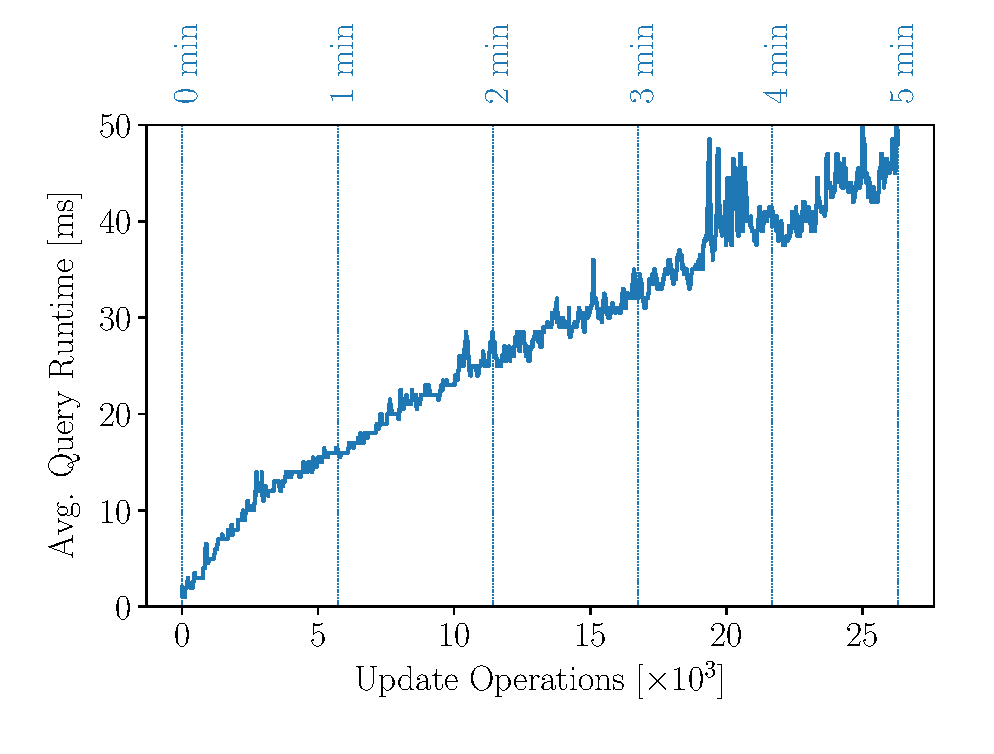
\includegraphics[height=3.8cm]{query_runtime.eps}
        \end{subfigure}
        \begin{subfigure}{0.45\textwidth}
            \centering
            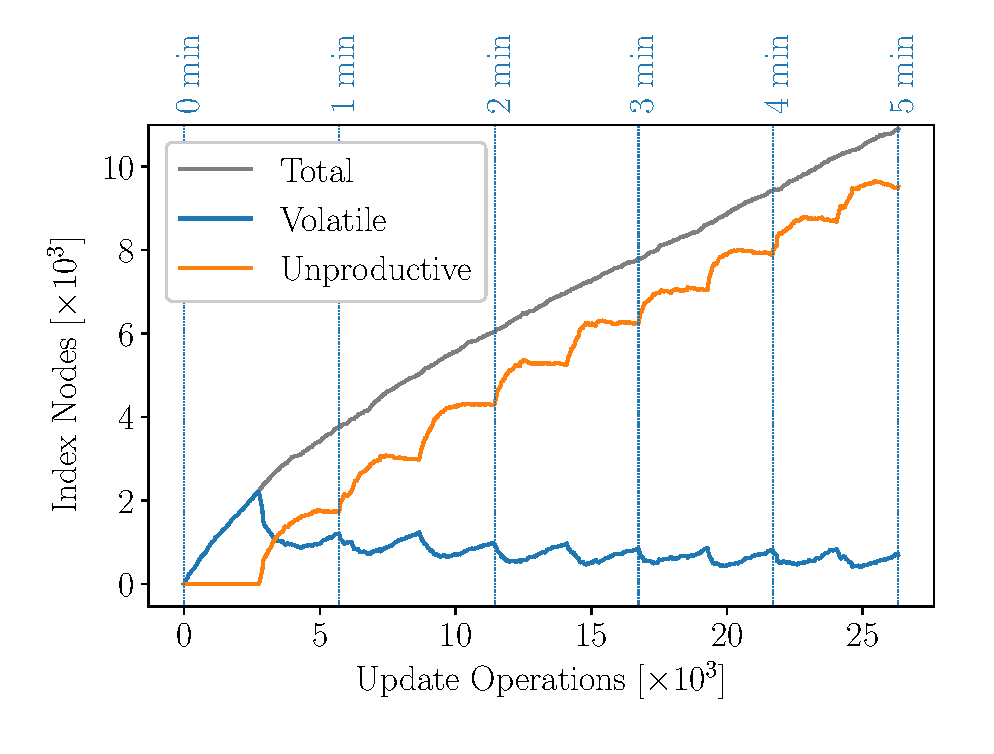
\includegraphics[height=3.8cm]{unprod_nodes.eps}
        \end{subfigure}
    \end{figure}
    \begin{itemize}
        \item Query runtime increases by an order of magnitude after five minutes
    \end{itemize}
}
\frame{
    \centering
    \large
    Volatility threshold $\tau$
}
\frame{
    \frametitle{Volatility threshold $\tau$} 
    \centering
    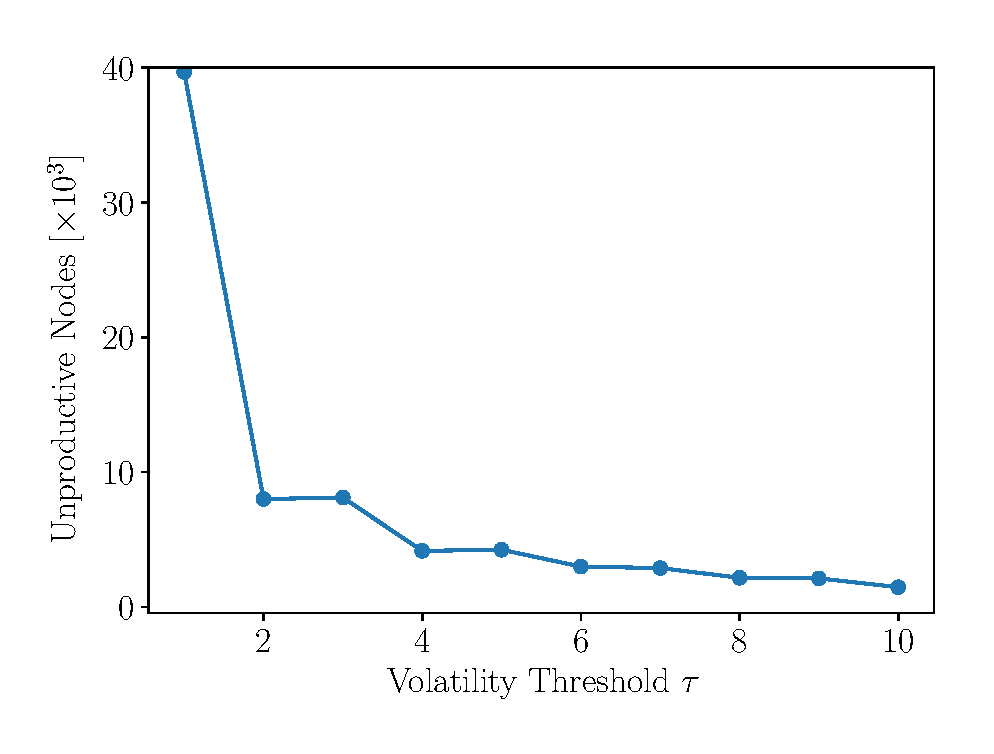
\includegraphics[height=5cm]{tau.eps}
}
\frame{
    \frametitle{Volatility threshold $\tau$} 
    \centering{
        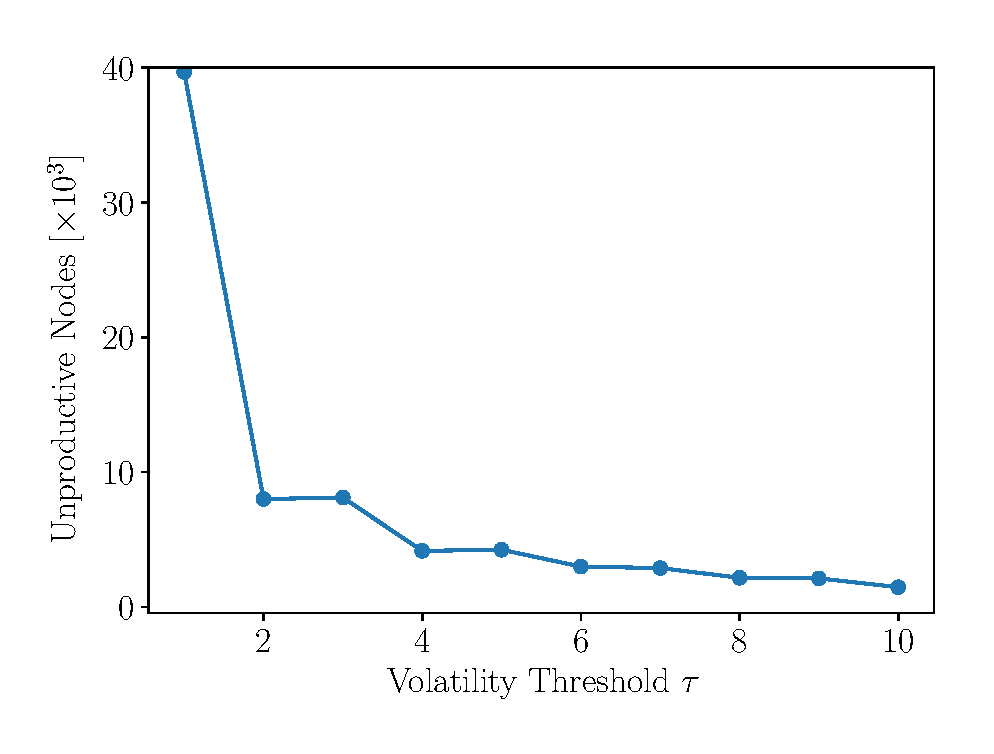
\includegraphics[height=4cm]{tau.eps}
    }
    \begin{itemize}
        \item $\tau \nearrow \quad \implies \text{volatile nodes} \searrow$
        \item volatile nodes $\searrow \quad \implies \text{unproductive nodes} \searrow$
        \item Power law relationship between \#unproductive nodes and $\tau$
    \end{itemize}
}
\frame{
    \centering
    \large
    Workload skew $s$
}
\frame{
    \frametitle{Workload skew $s$}
    \begin{figure}
        \centering
        \begin{subfigure}{0.30\textwidth}
            \centering
            \scriptsize
            \begin{forest}
                [,circle,draw,fill=YellowOrange
                [,circle,draw,fill=YellowOrange
                [,circle,draw,fill=YellowOrange
                ]
                [,circle,draw,fill=YellowOrange
                [,circle,draw,fill=YellowOrange]
                [,phantom]
                ]
                ]
                [,circle,draw,fill=YellowOrange
                [,phantom]
                [,circle,draw,fill=YellowOrange
                [,circle,draw,fill=YellowOrange]
                [,circle,draw,fill=YellowOrange]
                ]
                ]
                ]
            \end{forest}

            No skew

            $s = 0$
        \end{subfigure}
        \begin{subfigure}{0.30\textwidth}
            \centering
            \scriptsize
            \begin{forest}
                [,circle,draw,fill=Yellow
                [,circle,draw,fill=Yellow
                [,circle,draw,fill=Yellow
                ]
                [,circle,draw,fill=Yellow
                [,circle,draw,fill=Orange]
                [,phantom]
                ]
                ]
                [,circle,draw,fill=Orange
                [,phantom]
                [,circle,draw,fill=Yellow
                [,circle,draw,fill=Red]
                [,circle,draw,fill=Orange]
                ]
                ]
                ]
            \end{forest}

            Normal skew

            $s = 1$
        \end{subfigure}
        \begin{subfigure}{0.30\textwidth}
            \centering
            \scriptsize
            \begin{forest}
                [,circle,draw,fill=Yellow
                [,circle,draw,fill=Yellow
                [,circle,draw,fill=Yellow
                ]
                [,circle,draw,fill=Yellow
                [,circle,draw,fill=Yellow]
                [,phantom]
                ]
                ]
                [,circle,draw,fill=Yellow
                [,phantom]
                [,circle,draw,fill=Yellow
                [,circle,draw,fill=Red]
                [,circle,draw,fill=Red]
                ]
                ]
                ]
            \end{forest}

            High skew

            $s = 2$
        \end{subfigure}
    \end{figure}
}

\frame{
    \frametitle{Workload skew $s$}
    \centering
    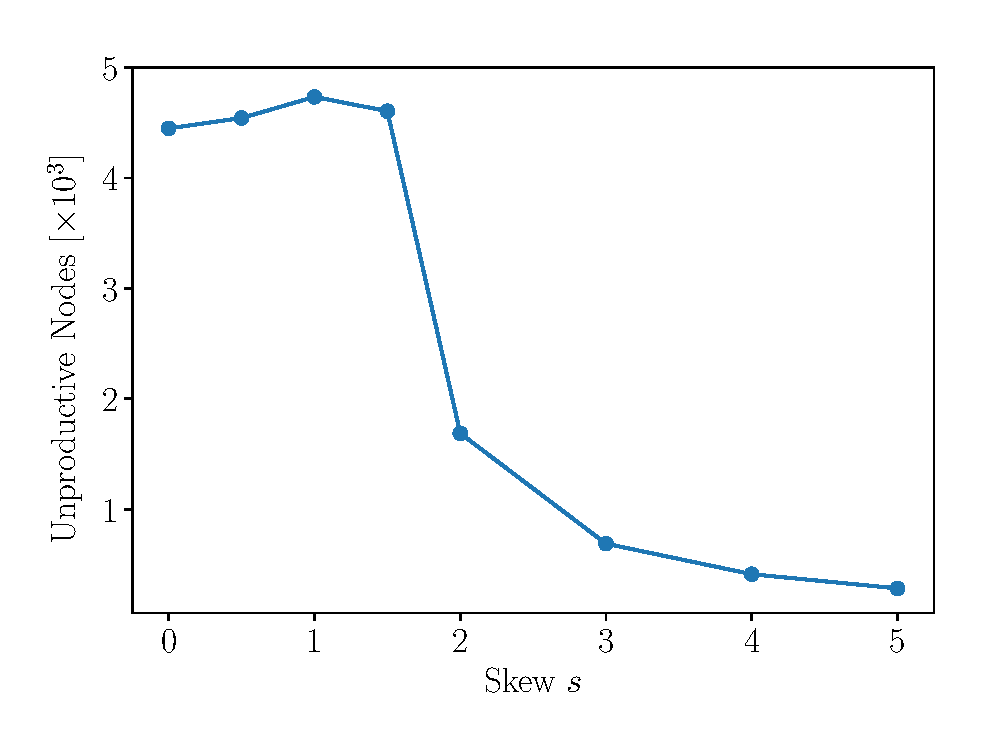
\includegraphics[height=5cm]{skew.eps}
}
\frame{
    \frametitle{Workload skew $s$} 
    \centering{
        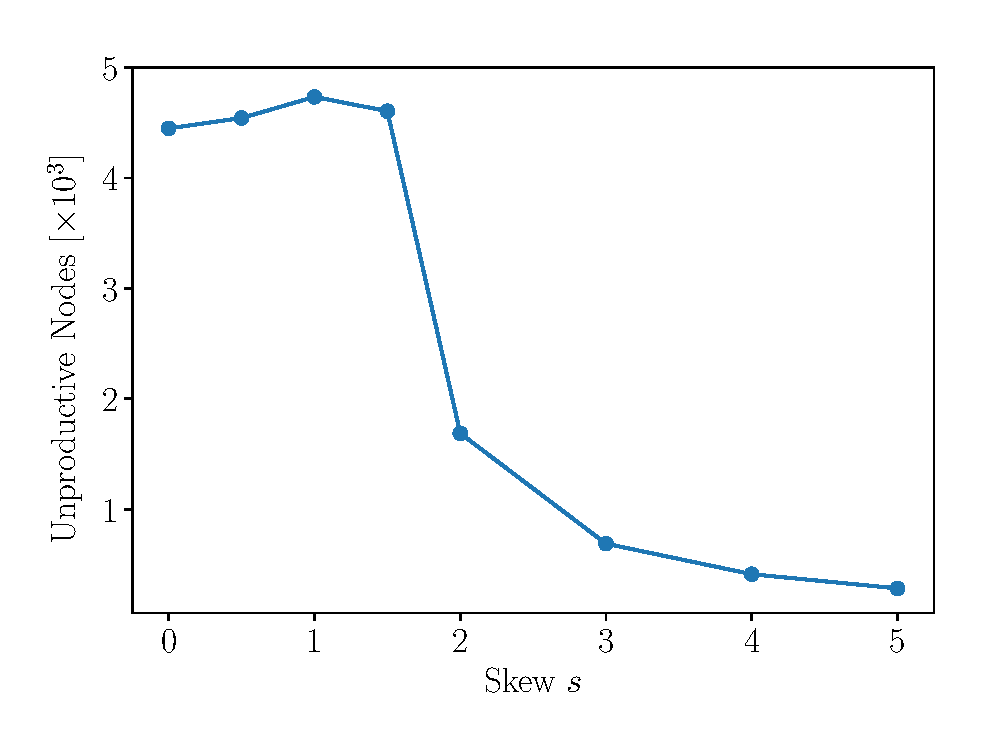
\includegraphics[height=4cm]{skew.eps}
    }
    \begin{itemize}
        \item $s > 1$ $\implies$ small hotspot $\implies$ few unproductive nodes
        \item $s < 1$ (uniform) $\implies$ no hotspot $\implies$ few unproductive nodes
    \end{itemize}
}
\subsection{Cleaning Unproductive Nodes}
\frame{
    \centering
    \large
    Cleaning Unproductive Nodes 
}
\frame{
    \begin{figure}
        \begin{subfigure}{0.45\textwidth}
            \centering
            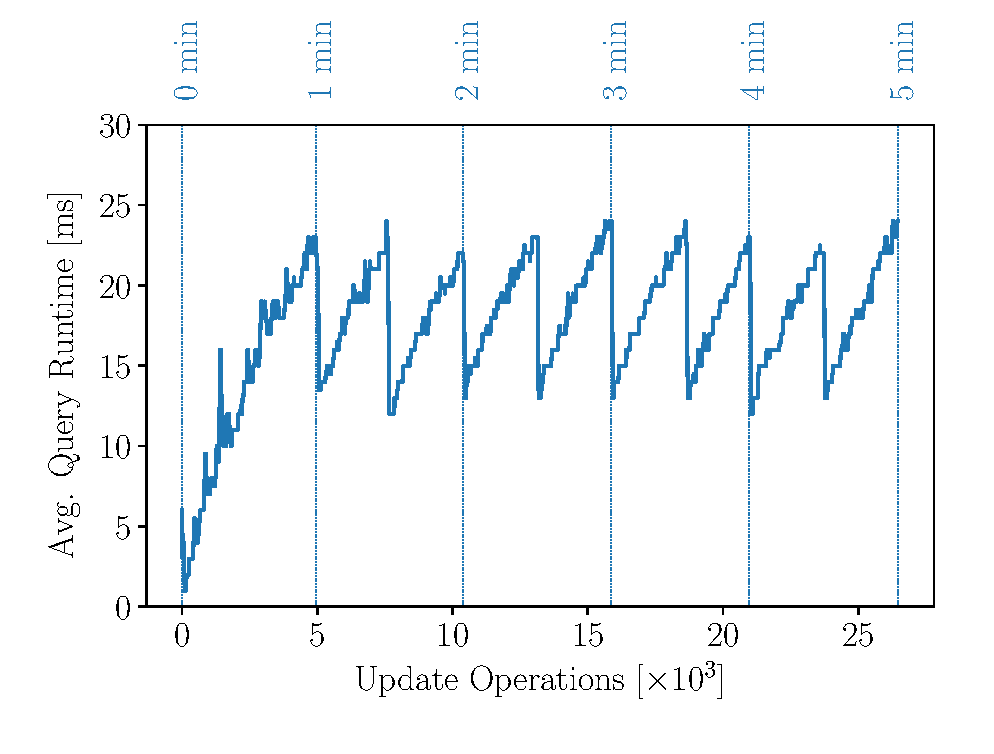
\includegraphics[height=3.8cm]{query_runtime_GC.eps}
        \end{subfigure}
        \begin{subfigure}{0.45\textwidth}
            \centering
            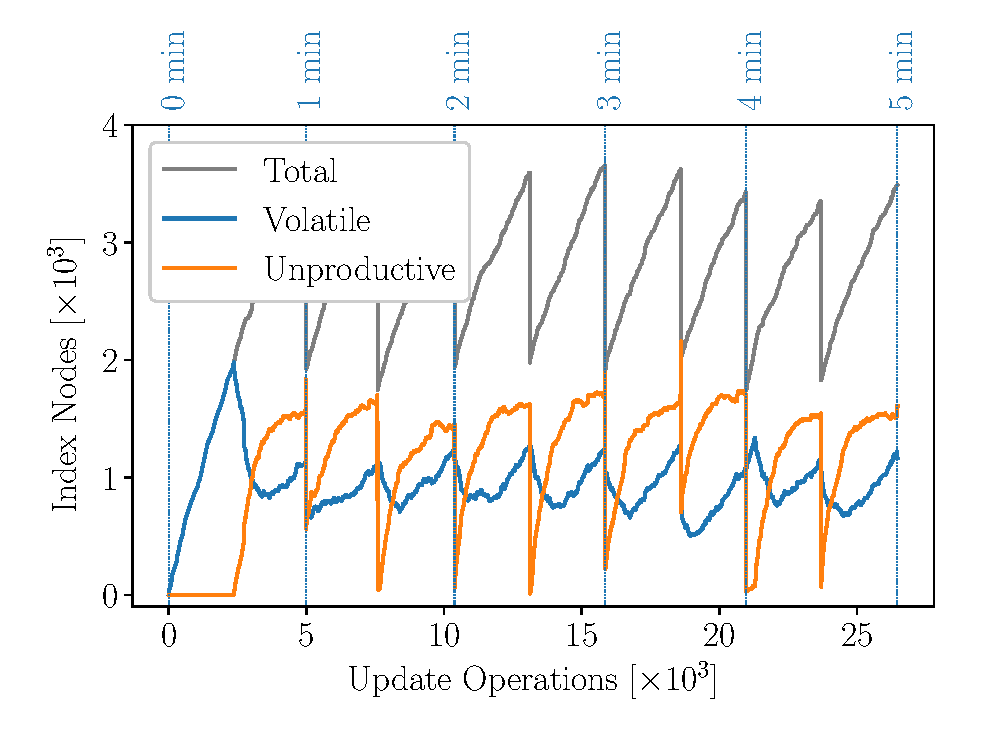
\includegraphics[height=3.8cm]{unprod_nodes_GC.eps}
        \end{subfigure}
    \end{figure}

    \centering
    \footnotesize
    We run GC every 30 seconds
    \vspace{3cm}
}
\frame{
    \begin{figure}
        \rotatebox{90}{GC}
        \begin{subfigure}{0.45\textwidth}
            \centering
            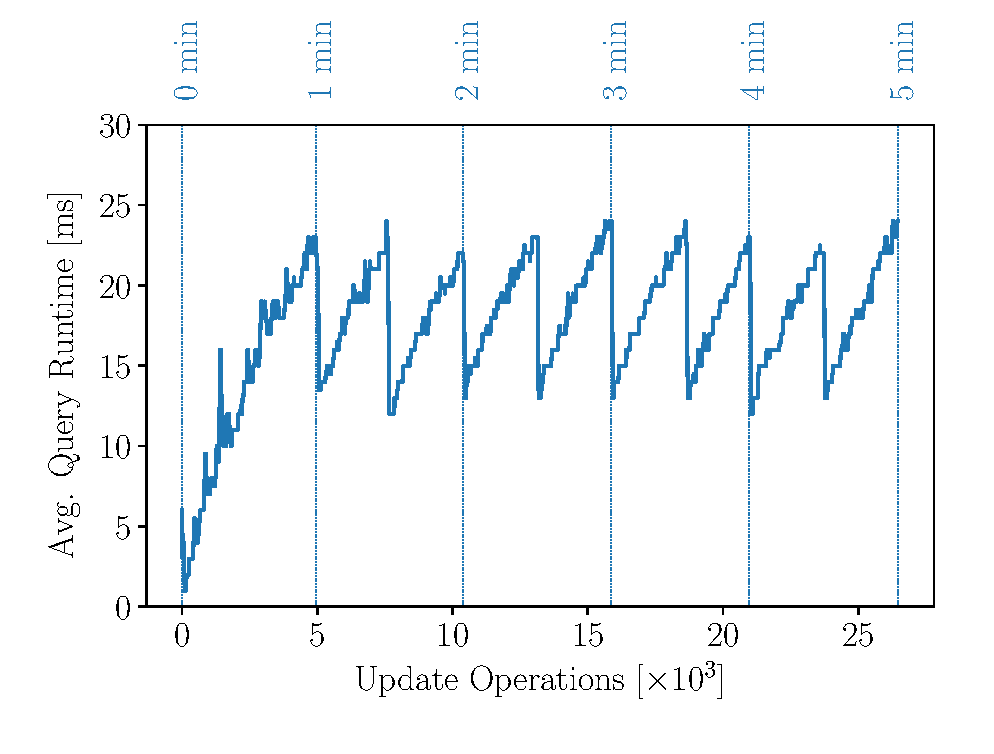
\includegraphics[height=3.8cm]{query_runtime_GC.eps}
        \end{subfigure}
        \begin{subfigure}{0.45\textwidth}
            \centering
            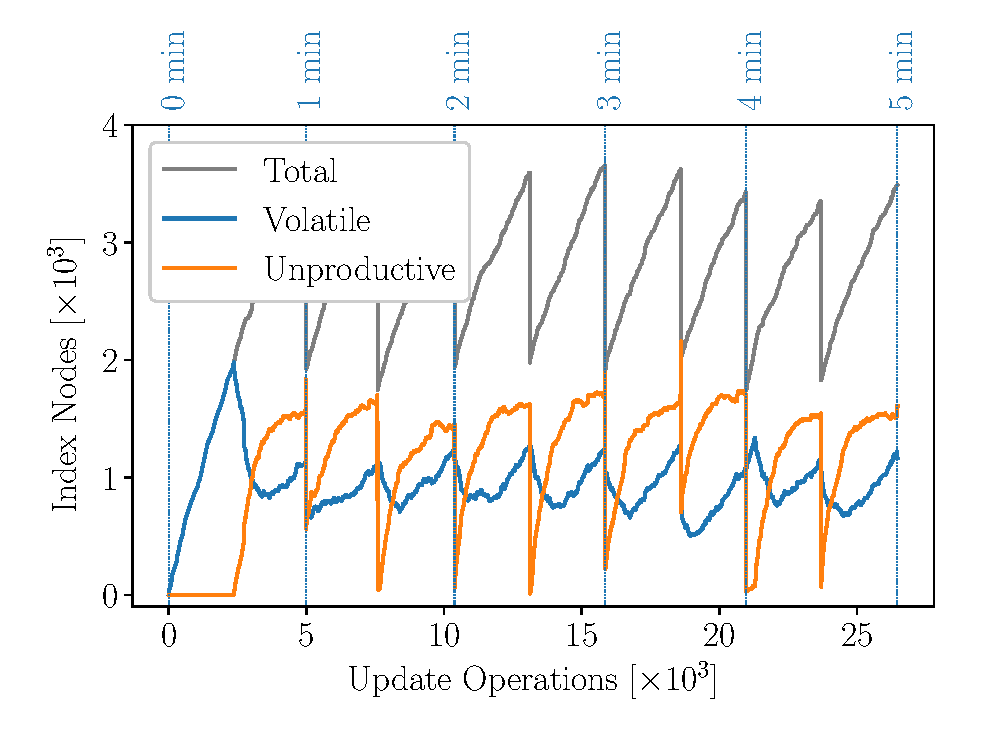
\includegraphics[height=3.8cm]{unprod_nodes_GC.eps}
        \end{subfigure}
    \end{figure}
    \vspace{-.5cm}
    \begin{figure}
        \rotatebox{90}{QTP}
        \begin{subfigure}{0.45\textwidth}
            \centering
            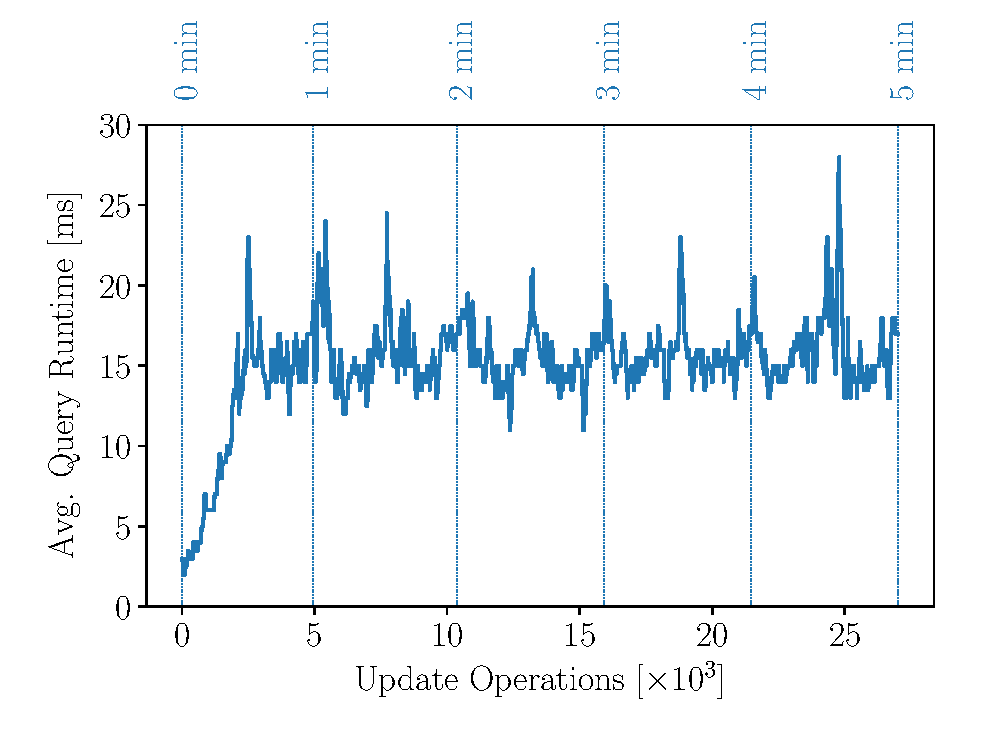
\includegraphics[height=3.8cm]{query_runtime_QTP.eps}
        \end{subfigure}
        \begin{subfigure}{0.45\textwidth}
            \centering
            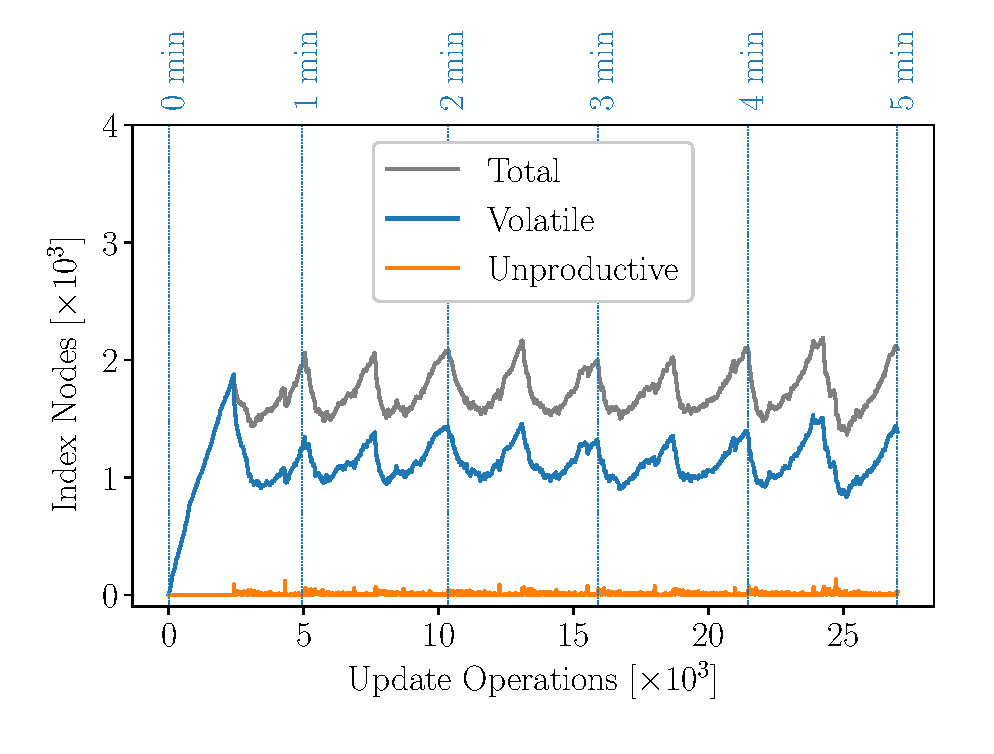
\includegraphics[height=3.8cm]{unprod_nodes_QTP.eps}
        \end{subfigure}
    \end{figure}
}

%\frame{
    %\frametitle{QTP}
    %\begin{figure}[H]
        %\centering
        %\begin{subfigure}{0.49\linewidth}
            %\centering
            %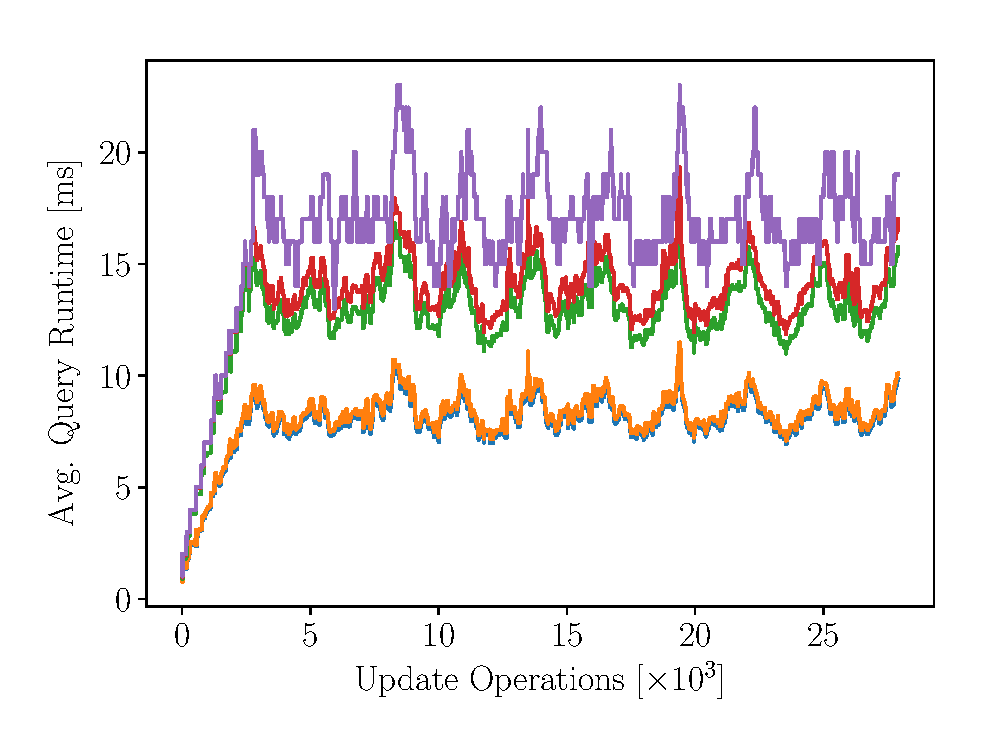
\includegraphics[width=6cm]{qtp_cost.eps}
        %\end{subfigure}
        %\begin{subfigure}{0.49\linewidth}
            %\centering
            %\begin{tikzpicture}[scale=0.52]
                %\fill[transparent] (-1,0) rectangle (0,5.5);
                %\filldraw[color=C0] (0,0) rectangle (1,2.40);
                %\filldraw[color=C1] (0,2.40) rectangle (1,2.56);
                %\filldraw[color=C2] (0,2.56) rectangle (1,4.01);
                %\filldraw[color=C3] (0,4.01) rectangle (1,4.31);
                %\filldraw[color=C4] (0,4.31) rectangle (1,5);
                %\fill[transparent] (0,5) rectangle (1,5.5);

                %\draw[dotted] (0.5,1.3) -- (5.5,0);
                %\node[align=left] at (6.7,0) {\footnotesize traversal};

                %\draw[dotted] (0.5,2.48) -- (5.5,1.25);
                %\node[align=left] at (7.1,1.25) {\footnotesize matching(n)};
                %\draw[dotted] (0.5,3.285) -- (5.5,2.5);
                %\node[align=left] at (7,2.5) {\footnotesize chd(n) = $\emptyset$};
                %\draw[dotted] (0.5,4.16) -- (5.5,4.5);
                %\node[align=left] at (6.9,4.5) {\footnotesize volatile(n)};
                %\draw[dotted] (0.5,4.66) -- (5.5,5.5);
                %\node[align=left] at (6.3,5.5) {\footnotesize write};
                %\draw [decorate,decoration={brace,amplitude=10pt,mirror,raise=4pt},yshift=0pt]
                %(1.1,2.56) -- (1.1,5.0) node [black,midway,xshift=1.8cm] {\footnotesize
                %QTP overhead};
            %\end{tikzpicture}
        %\end{subfigure}
    %\end{figure}
%}
\frame{
  \frametitle{GC period $T_{GC}$}
    \centering
    \begin{figure}
        \begin{subfigure}{0.45\textwidth}
            \centering
            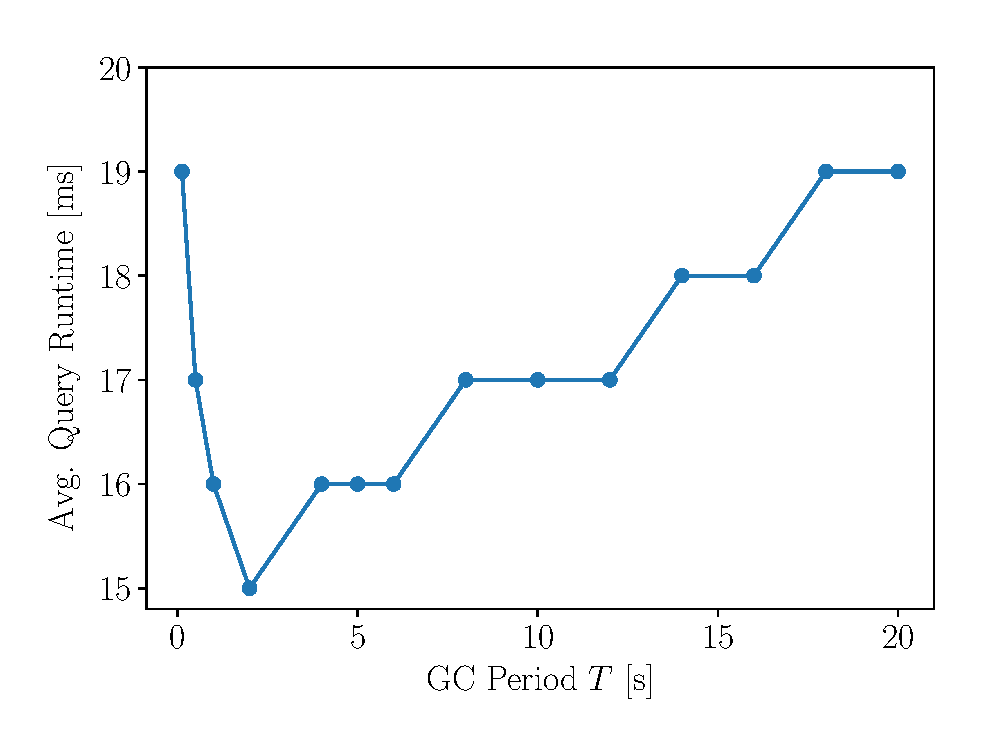
\includegraphics[height=3.8cm]{query_runtime_T.eps}
        \end{subfigure}
        \begin{subfigure}{0.45\textwidth}
            \centering
            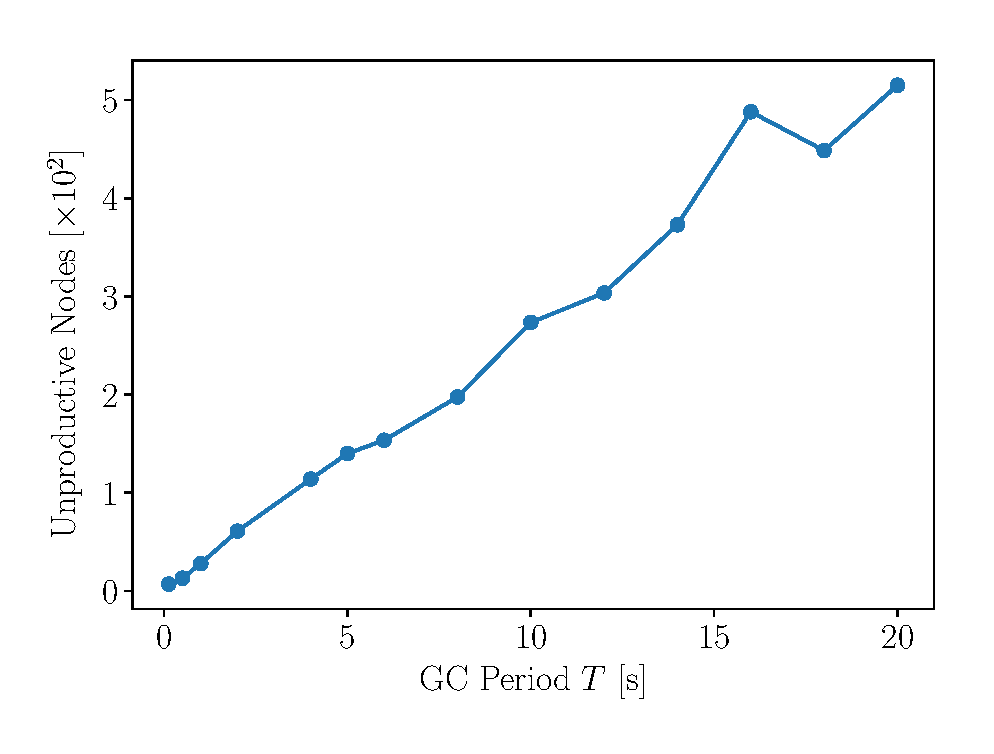
\includegraphics[height=3.8cm]{unprod_nodes_T.eps}
        \end{subfigure}
    \end{figure}

    \scriptsize
    \begin{itemize}
        \item Optimal GC period $T_{GC}^*$: period with the smallest query runtime
        \item Too small $T_{GC}$ $\implies$ GC steals resources from query executor
    \end{itemize}
}
\frame{
    \frametitle{QTP}
    \begin{figure}[H]
        \centering
        \begin{subfigure}{0.49\linewidth}
            \begin{algorithm}[H]
                \tiny{
                    \TitleOfAlgo{QueryQTP}
                    \DontPrintSemicolon
                    \KwData{Query $Q(k, v, m)$, where $k$ is a property, $v$ a value and $m$ (=
                        $\texttt{/}\lambda_1\texttt{/}\dots\texttt{/}\lambda_d$) a
                    content node's path.}
                    \KwResult{A set of nodes satisfying $Q(k,v,m)$}
                    $r \longleftarrow \emptyset$\;
                    \For{\textcolor{C2}{node $n \in
                      desc(\texttt{/i/k/v/}\lambda_1\texttt{/}\dots\texttt{/}\lambda_d)$} in postorder tree walk}{
                            \uIf{\textcolor{C2}{$matching(n)$}}{
                            $r \longleftarrow r \cup \{ *n \}$\;
                        }
                        \ElseIf{\textcolor{C0}{$children(n)$}$ = \emptyset \land \neg $\textcolor{C0}{$volatile(n)$}}{
                            \textcolor{C0}{delete} node $n$
                        }
                    }
                    \Return{r}\;
                }
            \end{algorithm}
        \end{subfigure}
        \begin{subfigure}{0.49\linewidth}
            \centering
            runtime [ms]
            \begin{tikzpicture}[scale=.6]
                \begin{axis}[
                    %xlabel = CPU time [$\mu$s],
                    xbar,
                    y axis line style = { opacity = 0  },
                    axis x line       = none,
                    %tickwidth         = 0pt,
                    %enlarge y limits  = 0.2,
                    %enlarge x limits  = 0.02,
                    symbolic y coords = {volatile 2.5\%,delete 15\%,children 30\%,matching 2.5\%,traversal 50\%},
                    nodes near coords,
                    ]
                    \addplot coordinates { 
                            (0.5,volatile 2.5\%) (3,delete 15\%)
                            (6,children 30\%) (0.5,matching 2.5\%)
                            (10,traversal 50\%) 
                        };
                \end{axis}
            \end{tikzpicture}
            %\begin{tikzpicture}[scale=0.5]
            %\fill[transparent] (-1,0) rectangle (0,5.5);
            %\filldraw[color=C0] (0,0) rectangle (1,2.40);
                %\filldraw[color=C1] (0,2.40) rectangle (1,2.56);
                %\filldraw[color=C2] (0,2.56) rectangle (1,4.01);
                %\filldraw[color=C3] (0,4.01) rectangle (1,4.31);
                %\filldraw[color=C4] (0,4.31) rectangle (1,5);
                %\fill[transparent] (0,5) rectangle (1,5.5);

                %\draw[dotted] (0.5,1.3) -- (5.5,0);
                %\node[align=left] at (6.7,0) {\footnotesize traversal};

                %\draw[dotted] (0.5,2.48) -- (5.5,1.25);
                %\node[align=left] at (7.1,1.25) {\footnotesize matching(n)};
                %\draw[dotted] (0.5,3.285) -- (5.5,2.5);
                %\node[align=left] at (7,2.5) {\footnotesize chd(n) = $\emptyset$};
                %\draw[dotted] (0.5,4.16) -- (5.5,4.5);
                %\node[align=left] at (6.9,4.5) {\footnotesize volatile(n)};
                %\draw[dotted] (0.5,4.66) -- (5.5,5.5);
                %\node[align=left] at (6.3,5.5) {\footnotesize write};
                %\draw [decorate,decoration={brace,amplitude=10pt,mirror,raise=4pt},yshift=0pt]
                %(1.1,2.56) -- (1.1,5.0) node [black,midway,xshift=1.8cm] {\footnotesize
                %QTP overhead};
            %\end{tikzpicture}
        \end{subfigure}
    \end{figure}
}
\subsection{Comparison}
\frame{
    \centering
    \Large
    Periodic GC vs.\ QTP
}
\frame{
    Simple model:

    \begin{itemize}
        \item assume constant rate of growth of unproductive nodes
    \end{itemize}
}
\frame{
    \frametitle{Simple Model}
    \begin{itemize}
        \item production rate of unproductive nodes \\
            $r = \frac{u}{s}$ ($u$ unproductive nodes per second)
    \end{itemize}

    \centering
    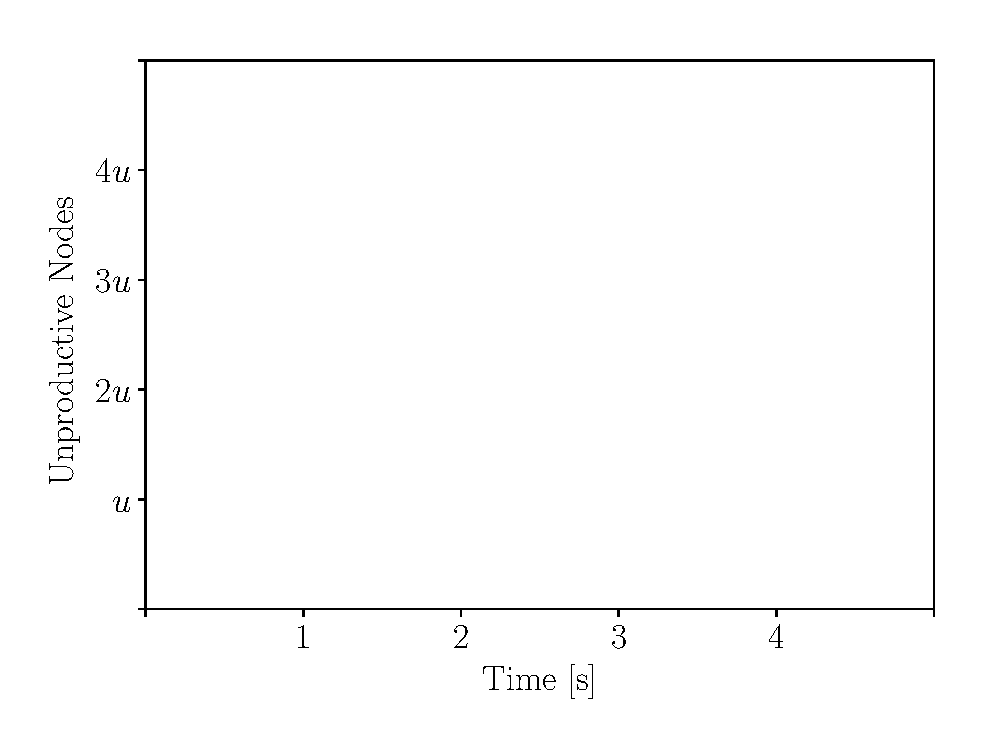
\includegraphics[width=7cm]{model_time.eps}
}
\frame{
    \frametitle{Simple Model, GC}
    \begin{itemize}
        \item production rate $r = \frac{u}{s}$
        \item GC period $T_{GC} = 2s$
    \end{itemize}

    \centering
    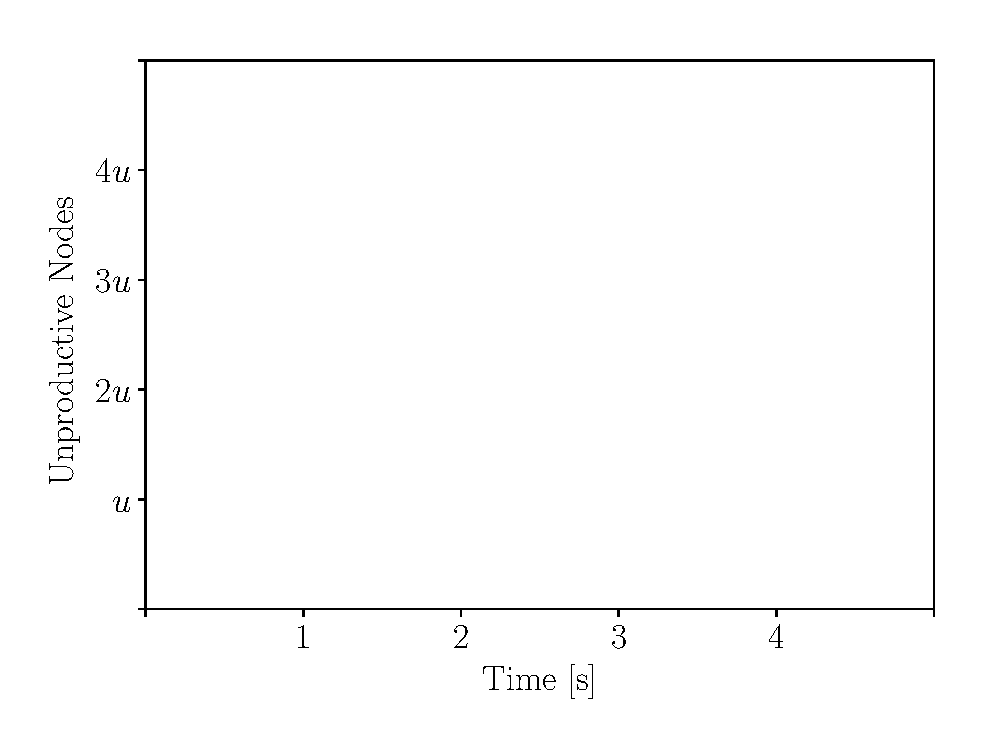
\includegraphics[width=7cm]{model_time.eps}
}
\frame{
    \frametitle{Simple Model, GC vs.\ QTP}
    \begin{itemize}
        \item production rate $r = \frac{u}{s}$
        \item GC period $T_{GC} = 2s$
    \end{itemize}

    \centering
    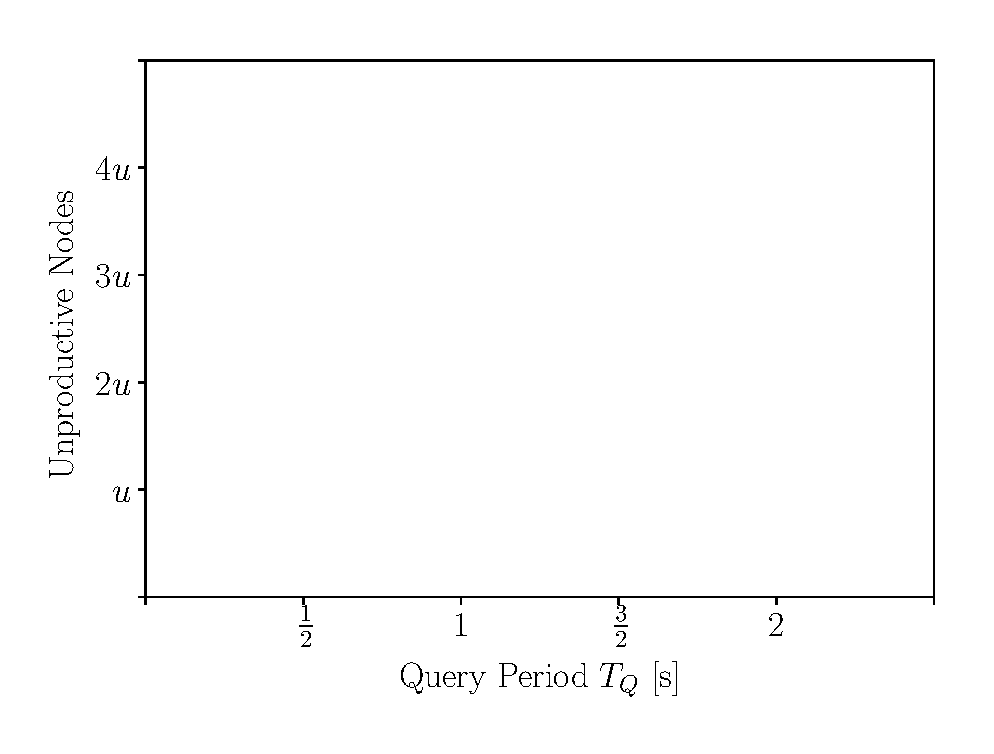
\includegraphics[width=7cm]{model_period.eps}
}
\frame{
    \frametitle{Simple Model, GC vs.\ QTP}
    \begin{itemize}
        \item production rate $r = \frac{u}{s}, r' = \frac{2 u}{s}$
        \item GC period $T_{GC} = 2s$
    \end{itemize}

    \centering
    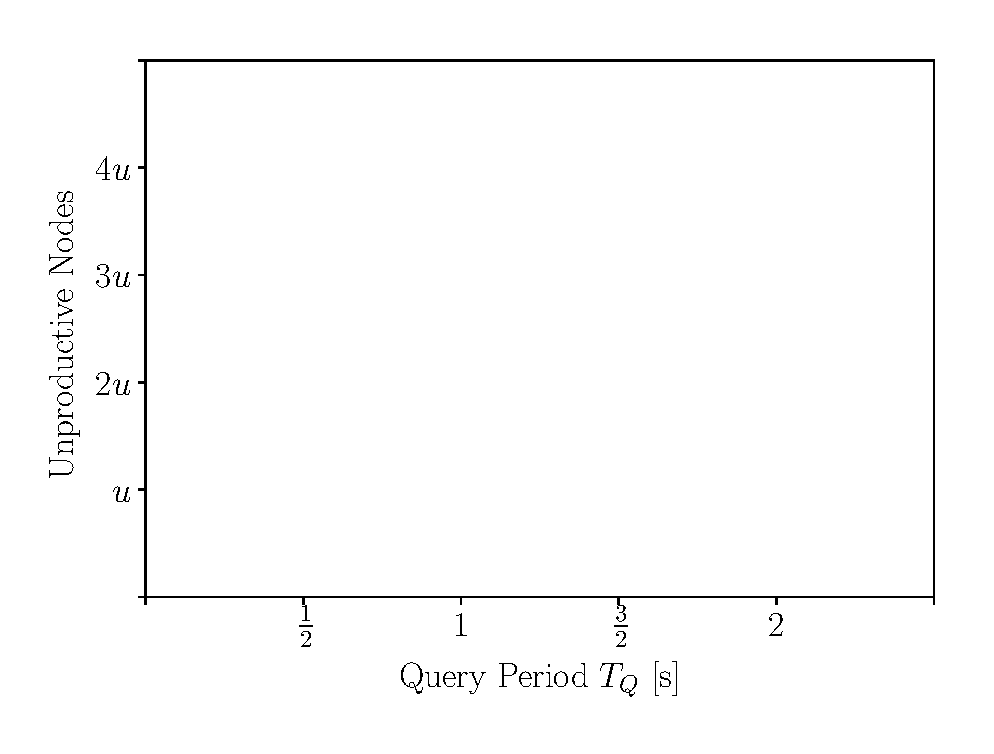
\includegraphics[width=7cm]{model_period.eps}
    }

%\frame{
    %\frametitle{GC vs.\ QTP, simple model}
    %\centering
    %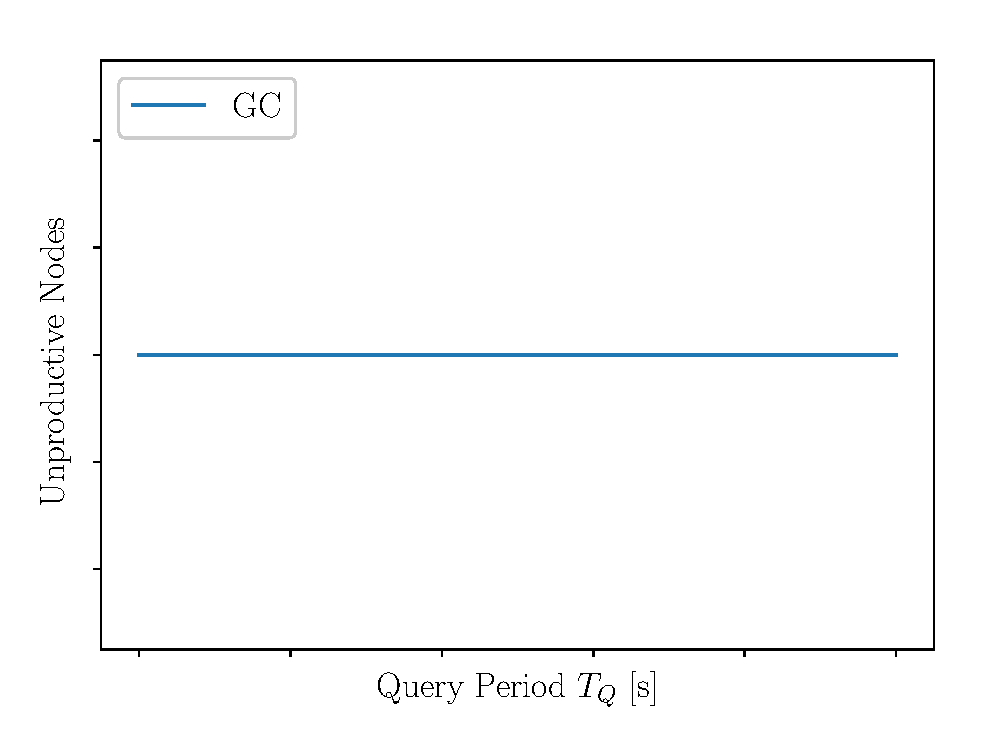
\includegraphics[width=7cm]{model_gc.eps}
%}
%\frame{
    %\frametitle{GC vs.\ QTP, simple model}
    %\centering
    %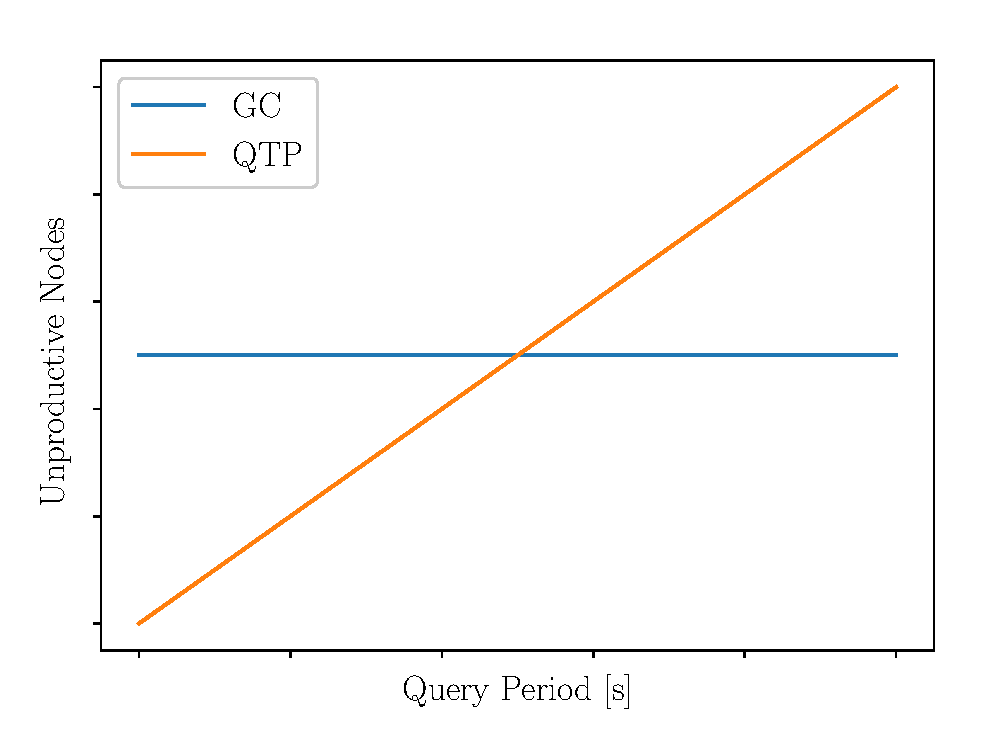
\includegraphics[width=7cm]{model_gc_qtp.eps}
%}
%\frame{
    %\frametitle{GC vs.\ QTP, simple model}
    %\centering
    %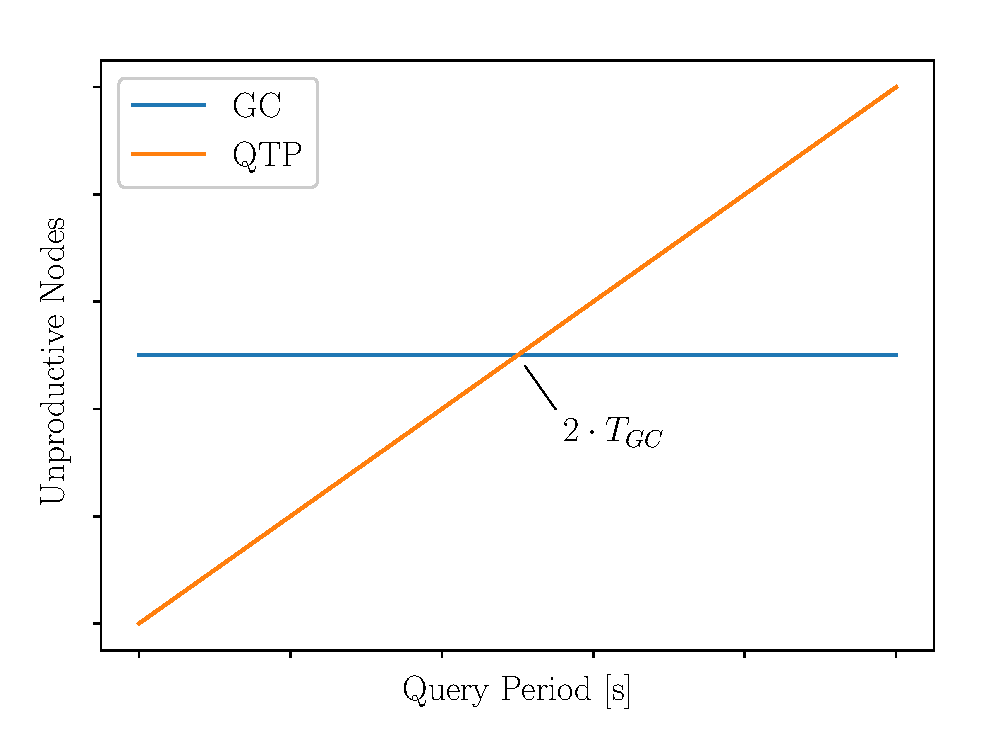
\includegraphics[width=7cm]{model_gc_qtp_equilibrium.eps}
%}
\frame{
    \frametitle{Simple Model, GC vs.\ QTP}
    \centering
    \begin{figure}
        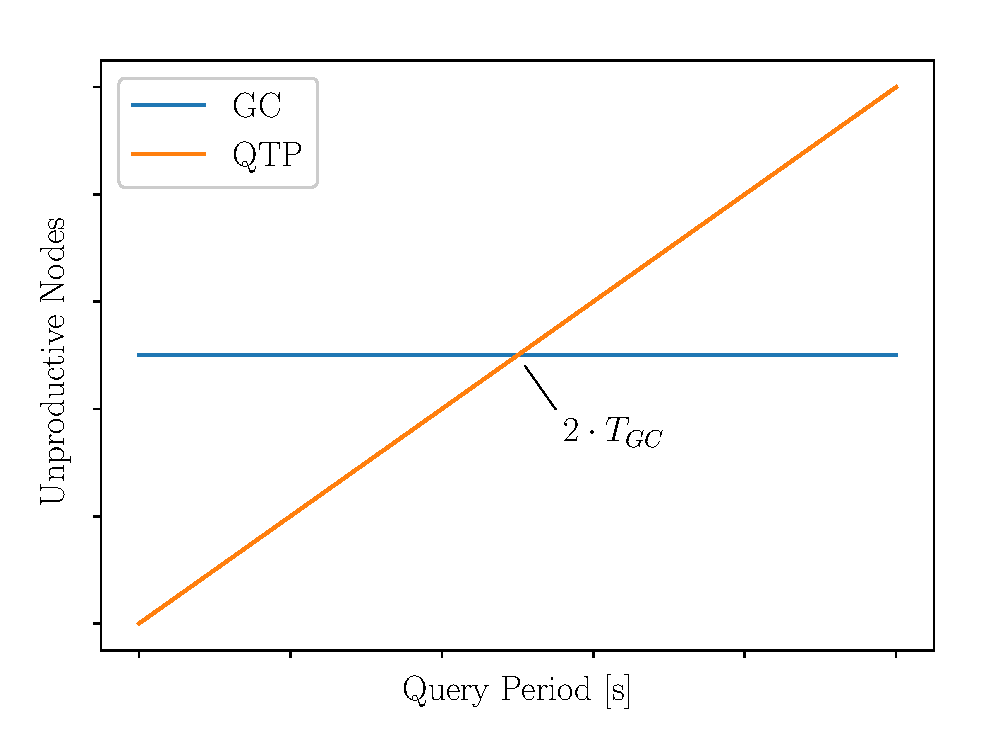
\includegraphics[height=5cm]{model_gc_qtp_equilibrium.eps}
    \end{figure}

    \footnotesize
    Queries traverse on average fewer unproductive nodes under QTP when
    the query period $T_Q$ is less than half the GC period $T_{GC}$

    %\large
    %$$ u_{GC} = u_{QTP} \iff T_Q = \frac{T_{GC}}{2} $$
}
\frame{
    \begin{figure}
        \centering
        \begin{tikzpicture}[node distance=1.2cm]
            \node (start) [startstop] {Start};
            \node (GCperiod) [process, below of=start] {Find optimal GC period $T_{GC}^*$};
            \node (Qperiod) [process, below of=GCperiod] {Find query period $T_Q$};
            \node (dec) [decision, below of=Qperiod, node distance=1.7cm] {$T_Q > \frac{T_{GC}^*}{2}$};
            \node (GC) [process, left of=dec, node distance=4cm] {Pick GC};
            \node (QTP) [process, right of=dec, node distance=4cm] {Pick QTP};
            \node (stop) [startstop, below of=dec, node distance=1.5cm] {Stop};

            \draw [arrow] (start) -- (GCperiod);
            \draw [arrow] (GCperiod) -- (Qperiod);
            \draw [arrow] (Qperiod) -- (dec);
            \draw [arrow] (dec) -- node [anchor=south,near start] {Yes} (GC);
            \draw [arrow] (dec) -- node [anchor=south,near start] {No} (QTP);
            \draw [arrow] (GC) |- (stop);
            \draw [arrow] (QTP) |- (stop);
        \end{tikzpicture}
    \end{figure}
}
%\frame{
    %\frametitle{GC vs.\ QTP}
    %\centering
    %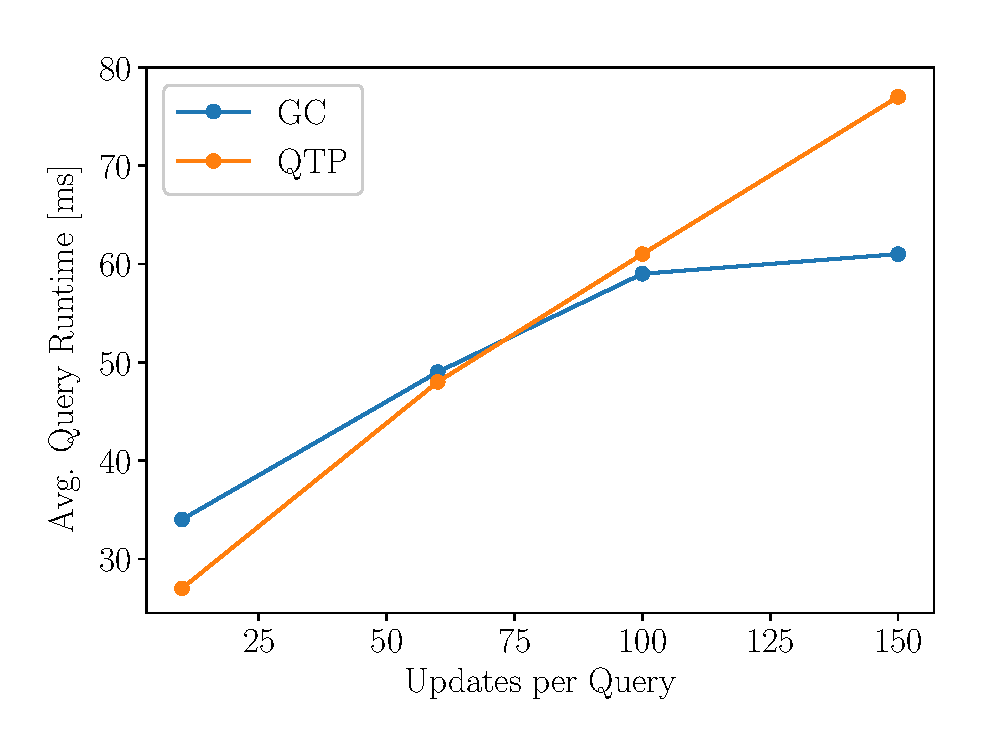
\includegraphics[width=7cm]{gc_vs_qtp.eps}
%}
%\subsection{Subsection 1}
%\frame{
    %\frametitle{frame title}
    %\begin{block}{Block title}
        %Block contents
    %\end{block}
    %\begin{itemize}
        %\item item1
        %\item item2
    %\end{itemize}
%}

\section{Conclusion}
\subsection{Summary}
\frame{
    \centering
    \Large
    Conclusion
}
\frame{
    \frametitle{Unproductive Nodes}
    \begin{itemize}
        \item volatility threshold $\tau \nearrow \enspace \implies$ unproductive nodes $\searrow$
        \item sliding window length $L \nearrow \enspace \implies$ unproductive nodes $\nearrow$
        \item workload skew $s \uparrow \downarrow \enspace \implies$ unproductive nodes $\searrow$
        \item update operations per second $ \nearrow \enspace \implies$ unproductive nodes $\nearrow$
    \end{itemize}
}
\frame{
    \frametitle{GC \& QTP}
    GC
    \begin{itemize}
        \item Periodically cleans unproductive index nodes 
        \item Sawtooth pattern
        \item Slows down system if run too often
    \end{itemize}

    QTP
    \begin{itemize}
        \item Faster and more stable than GC when queries are frequent
        \item Adds overhead to queries
        \item Overhead negligible in the long-term
    \end{itemize}
}
\subsection{Future Work}
\frame{
    \centering
    \Large
    Future Work
}
\frame{
    \frametitle{Future Work}
    \begin{itemize}
        \item Concurrency control
        \item Frequently changing query filter
        \item Unproductive node production rate
    \end{itemize}
}   
%\subsection{References}
%\frame{
    %\frametitle{References}
    %\scriptsize
    %\bibliography{bib}
%}

\end{document}
